\chapter{Analyse}

\section{Logoot}
	\emph{logoot} est un algorithme destiné à l'édition de documents textes sur
	un réseau \emph{peer-to-peer} (cf. \ref{sec:p2p}). Concrètement, cet
	algorithme permet de partager la position des caractères du document entre
	les différentes personnes travaillant dessus.
	
	\subsection{Fonctionnement}
		Chaque utilisateur possède un tableau dans lequel y est placé la
		position de tous les caractères du document collaboratif. Lorsqu'un
		caractère est ajouté par un utilisateur, ce dernier est envoyé à travers
		le réseau afin que chaque autre utilisateur puisse mettre à jour son
		tableau et le document.\\
		
		Initialement
			
	\subsection{Algorithme}
		

\section{Peer-to-Peer}\label{sec:p2p}

	Un réseau peer-to-peer est un modèle ou chaque client est aussi serveur. En
	effet, dans un réseau peer-to-peer, l'information est diffusée au travers du
	réseau grâce aux clients qui relaient l'information. Comme représenté en
	figure \ref{fig:p2p} page \pageref{fig:p2p}, le réseau est décentralisé,
	chaque ordinateur joue un double rôle de client et de serveur. L'avantage
	d'un tel réseau est qu'il soit décentralisé, en effet, la vie d'une
	ressource ne repose pas sur un seul serveur (comme c'est le cas dans un
	réseau classique) mais bien sûr tous les éléments du réseau qui la possède.
	Ainsi, même si l'un des noeuds cesse d'émettre, la ressource reste
	disponible via les autres noeuds qui la possède.
	
	\begin{figure}
	  \center
      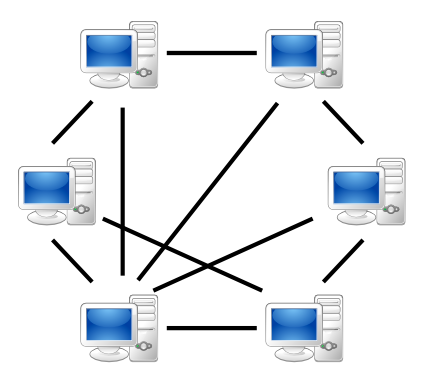
\includegraphics[width=0.4\textwidth]{includes/P2P-network.png}
      \caption{Exemple de réseau peer to peer}
      \label{fig:p2p}
    \end{figure}
	
	\subsection{Gossip}
	
		Gossip est un protocole de communication basé sur l'idée
		d'\emph{épidémie} ou de rumeur: une personne lance une rumeur à ses
		voisins qui eux-même la disent à leurs voisins, etc au bout d'un certain
		temps, toutes personnes connaissent la rumeur lancée par une celle
		d'origine.
		
		L'avantage d'utiliser \emph{Gossip} est qu'il permet de fonctionner dans
		un réseau non structuré. En effet, en utilisant \emph{Gossip}, il n'est
		pas nécessaire de connaitre la structure du réseau pour pouvoir
		fonctionner.
		
		On suppose que l'on souhaite faire la recherche d'un ressource X qui se
		trouve sur l'un des postes du réseau, le principe du protocole est le
		suivant:
		\begin{enumerate}
			\item Chaque noeud possède une liste de \emph{peer} dans le réseau.
			\item À intervale régulier, le poste prend un peer au hazard dans la
			liste et lui envoie le message.
			\item Le poste qui reçoit le message vérifie s'il possède la
			ressource: si c'est le cas, il répond, sinon il recommence depuis
			l'étape 2 et ainsi de suite.
		\end{enumerate}~
		De cette façon, en un temps logarithmique, chaque noeud du réseau aura
		reçu le message et l'initiateur de la recherche aura donc la réponse. À
		chaque "tour", le nombre de personne renvoyant le message est doublé ce
		qui rend le protocole très robuste car, même si un message est perdu en
		cours de route, le noeud qui aura manqué ce message, le recevra de la
		part d'un autre peer.\\
		
		Ce protocole est la solution pour le projet. En effet, le réseau sur
		lequel les personnes font le travail collaboratif n'est pas connu et
		encore moins structuré. Une implémentation java est disponible par
		l'Inria, cependant lors de la recherche d'un protocole peer-to-peer, ce
		dernier était encore en cours de développement ce qui rendait son
		utilisation très difficile, de plus, la pauvreté de documentation
		concernant le code ne facilitait pas la tâche d'apprentissage. C'est
		pour cela que nous n'avons pas retenu \emph{Gossip} pour le réseau
		peer-to-peer
	
	\subsection{Jxta}
		JXTA est une technologie open source permettant de faire un réseau
		peer-to-peer en Java. Le principe est simple, un réseau peer-to-peer est
		créé sur le réseau existant permettant aux différents noeuds de pouvoir
		communiquer entre eux.\\
		
		Étant un projet connu, la communauté derrière cette technologie et
		l'abondante documentation ont permis de choisir et d'utiliser
		\emph{Jxta} assez facilement.